\section{Experiments}
\label{sec:experiments}

We evaluate TransitDuet on an event-driven bus microsimulation against three external baselines and six component ablations.
All results are from three independent random seeds.

%% ============================================================
\subsection{Experimental setup}
\label{sec:exp_setup}

\paragraph{Simulation environment.}
We implement an event-driven bus simulation modeling a single bidirectional route with 22 stations (11 per direction), serving 264 scheduled trips per day.
Passenger demand follows origin--destination (OD) matrices with time-varying arrival rates calibrated to reproduce morning and evening peaks.
The simulation advances at a resolution of $\Delta t = 1$\,s.
Passenger arrivals and alighting events are updated every 20\,s. The upper-level planner is event-driven --- it is invoked once per dispatch event (a total of 264 events per simulated service day, $\approx 132$ per direction; the inter-event interval is the realised dispatch headway, not a fixed timer), and the lower-level holding controller is invoked once per station arrival.
Travel times between consecutive stations are drawn from log-normal distributions whose parameters vary by time of day and direction, with a route stochasticity parameter $\sigma$ controlling variance (default $\sigma_{\mathrm{route}} =1.5$).

\paragraph{Methods.}
We evaluate TransitDuet against three external baselines and six component ablations.
All methods operate on the same environment with demand stochasticity
(per-hour multiplier $\mathcal{N}(1, 0.15^2)$, clipped to $[0.3, 2.0]$)
and elastic fleet budget $\Nfleet \sim \mathrm{Uniform}[8, 16]$ sampled per episode.

\noindent\textit{External baselines:}
\begin{itemize}[leftmargin=*]
    \item \textbf{Fixed}: static timetable with $H = 360$\,s throughout the day; only the lower-level holding controller is trained. A strong hand-tuned baseline.
    \item \textbf{GA}: genetic-algorithm search over $[\Hpeak, \Hoff, \Htrans]$ (pop\,size\,15, $\sigma_{\text{mut}}=0.15$).
    \item \textbf{CMA-ES}: covariance-matrix adaptation evolution strategy (pop\,size\,10, $\sigma_0 = 0.3$).
\end{itemize}

\paragraph{Baseline fairness.}
All four methods (Fixed, GA, CMA-ES, TransitDuet) use the same lower-level RE-SAC Lagrangian holding controller architecture (hidden dim, ensemble size, $\beta_{\mathrm{LCB}}$, action range, cost limit, soft-update rate) and the same elastic-fleet sampling. The training budget is approximately matched: TransitDuet and the static Fixed baseline both train for 300 episodes per seed, while the search baselines (GA, CMA-ES) run a 20-episode lower-only warmup followed by 300 search-evaluation episodes (320 simulator episodes total, $+6.7\%$ vs.~TransitDuet) --- the warmup is needed because their upper search starts only after the lower has stabilised, whereas the Fixed baseline has no upper search and skips the warmup; we have aligned the lower hyperparameters used by the baselines with the \texttt{H\_hiro} main run ($\lambda_{\mathrm{lr}} = 10^{-4}$, $\alpha_{\max}^{\mathrm L} = 0.1$). This is a near-unified protocol rather than an exact one --- see \cref{sec:discussion} for a discussion of the residual differences. Concretely: each method trains a single shared lower controller end-to-end against its upper, so the comparison isolates the effect of the upper-level decision rule rather than confounding it with a different lower-controller architecture. For GA and CMA-ES, we run a single search loop (one population that evolves in place), evaluating each candidate timetable triple with the shared lower controller; the population size and per-candidate evaluation budget are tuned so the total wall-clock training cost matches that of TransitDuet to within $5\%$. We do not retrain the lower controller per candidate (which would 15--30$\times$ the GA/CMA-ES cost); instead, both search baselines share the same lower training schedule as TransitDuet. We acknowledge this is a soft choice: a search baseline given a per-candidate dedicated lower training budget might close some of the gap to TransitDuet, at correspondingly higher cost. Stronger baselines such as MPC / rolling-horizon optimisation and time-of-day MILP are out of scope here and discussed in~\Cref{sec:discussion}.

\noindent\textit{Component ablations} (all start from TransitDuet full):
\begin{itemize}[leftmargin=*]
    \item \textbf{--HoldFB}: remove holding-feedback coupling from the upper state (state dims $5$--$7$ zeroed).
    \item \textbf{--CS-BAPR}: disable the Bayesian changepoint belief tracker; upper $\alpha$ stays at nominal value.
    \item \textbf{--Hindsight}: disable the per-dispatch gap-deviation credit; upper uses only episode-level system reward.
    \item \textbf{--MORL}: replace belief-weighted $\thetavec$-OGD scalarization with fixed weights $[0.5, 0.25, 0.25]$.
    \item \textbf{--Elastic}: fix $\Nfleet = 12$ during training (policy does not see elastic budget).
    \item \textbf{--DemandNoise}: deterministic demand (remove the per-hour multiplier and peak-time shift).
\end{itemize}

\paragraph{Metrics.}
For each method and seed we select the validation-best checkpoint via held-out evaluation (six checkpoints per training run at episodes \{49, 99, 149, 199, 249, 299\}; for each checkpoint we run 20 fresh evaluation episodes drawn from the same simulator distribution as training, and pick the checkpoint that minimises mean composite cost). Reported metrics are then aggregated as 3-seed mean $\pm$ std over the per-seed validation-best checkpoints:
\begin{itemize}
    \item \emph{Average passenger wait time} (min): time between a passenger's arrival at a station and boarding.
    \item \emph{Headway coefficient of variation} (CV): $\sigma_h / \mu_h$ across inter-dispatch gaps within an episode; captures regularity.
    \item \emph{Fleet overshoot}: $\max(0, \text{peak fleet} - \Nfleet)$; non-zero when the policy exceeds the sampled budget.
    \item \emph{Composite cost}: $\mathrm{wait}/10 + \mathrm{overshoot}^2 / \Nfleet + \mathrm{CV}$, the upper-level training objective. Lower is better on all four.
\end{itemize}

\paragraph{Training protocol.}
TransitDuet, the HIRO ablations and the Fixed baseline are trained for 300 episodes per seed with three independent random seeds; the search baselines (GA, CMA-ES) use a 20-episode lower-only warmup followed by 300 search-evaluation episodes (320 simulator episodes total, $+6.7\%$ over TransitDuet) under otherwise identical lower hyperparameters --- a near-unified, approximately budget-matched protocol rather than an exact one (see \cref{sec:discussion}).
We report means and standard deviations across seeds.

\paragraph{Hyperparameters.}
\Cref{tab:hyperparams} summarizes the key hyperparameters.
All values are shared across methods where applicable; method-specific ablations disable the corresponding component as described above.

\begin{table*}[t]
\centering
\caption{Hyperparameters for TransitDuet (values match \texttt{config\_v2.yaml} in the released code).}
\label{tab:hyperparams}
\begin{tabular}{@{}llr@{}}
\toprule
\textbf{Component} & \textbf{Parameter} & \textbf{Value} \\
\midrule
Upper policy   & Hidden dim                                   & 64 \\
               & Learning rate                                & $3 \times 10^{-4}$ \\
               & Discount factor $\gamma_{\mathrm U}$         & 0.95 \\
               & Batch size                                   & 64 \\
               & Updates / episode                            & 10 \\
               & Replay capacity                              & 50{,}000 \\
               & Ensemble size $K$                            & 10 \\
               & LCB coefficient $\beta_{\mathrm{LCB}}$       & $-2.0$ \\
               & Action range $\delta_{\max}$                 & 120 s \\
               & Maximum entropy temperature $\alpha_{\max}^{\mathrm U}$ & 0.05 \\
\midrule
Lower policy   & Hidden dim                                   & 64 \\
               & Learning rate                                & $3 \times 10^{-4}$ \\
               & Discount factor $\gamma_{\mathrm L}$         & 0.99 \\
               & Batch size                                   & 512 \\
               & Updates / episode                            & 30 \\
               & Replay capacity                              & 500{,}000 \\
               & Ensemble size $K$                            & 10 \\
               & LCB coefficient $\beta_{\mathrm{LCB}}$       & $-2.0$ \\
               & OOD spread weight $\beta_{\mathrm{ood}}$     & 0.1 \\
               & Soft-update coefficient $\tau$               & 0.005 \\
               & Action range                                 & 60 s \\
               & Reward scale                                 & 1.0 \\
               & Maximum entropy temperature $\alpha_{\max}^{\mathrm L}$ & 0.1 \\
\midrule
Lagrangian     & Cost limit $\climit$                          & 0.5 \\
               & Dual variable learning rate $\lambda_{\mathrm{lr}}$ & $1 \times 10^{-4}$ \\
\midrule
Coupling sched.& Lower-only warmup                            & 30 episodes \\
               & Hindsight credit weight $\alpha_{\mathrm H}$ & 0.5 \\
               & TPC behaviour mix $\epsilon$                 & 0.25 \\
               & TPC target std $\sigma_{\mathrm{tgt}}$       & 20 s \\
               & TPC IS clip $w_{\max}$                       & 5 \\
               & TPC EMA Polyak rate $\tau$                   & 0.005 \\
\midrule
Fleet          & Default $\Nfleet$ (fixed mode)               & 12 \\
               & Elastic range                                & $[8, 16]$ \\
\midrule
Training       & Episodes per seed                            & 300 \\
\bottomrule
\end{tabular}
\end{table*}

%% ============================================================
\subsection{Main results}
\label{sec:main_results}

\Cref{tab:main_results} compares TransitDuet against three external baselines.

\begin{table*}[t]
\centering
\caption{Main comparison under a near-unified, approximately budget-matched evaluation protocol (demand noise 0.15, elastic $\Nfleet \in [8, 16]$, 3 seeds). TransitDuet, the HIRO ablations and the Fixed baseline train for 300 episodes per seed; the search baselines (GA, CMA-ES) train for 20 lower-only warmup + 300 search-evaluation episodes (320 simulator episodes total per seed). All methods share the same lower-level RE-SAC--Lagrangian holding controller architecture and hyperparameters. For TransitDuet and the HIRO ablations we report the validation-selected checkpoint per seed (20 fresh eval episodes per checkpoint, best by composite cost). For GA and CMA-ES we report the validation-best lower checkpoint paired with the search's final upper triple, which is a softer pairing; see \cref{sec:discussion}. For the 3-seed learned-lower rows (Fixed, GA, CMA-ES, TransitDuet) the $\pm$ values denote 3-seed std; for the 1-seed Rule-MPC / Rule-GA / Rule-CMA-ES / Per-cand-GA sanity-check rows the $\pm$ values denote held-out episode std (n=20). Lower is better on all four metrics; best in \textbf{bold}.}
\label{tab:main_results}
\begin{tabular}{@{}lcccc@{}}
\toprule
\textbf{Method} & \textbf{Wait (min)} & \textbf{CV} & \textbf{Overshoot} & \textbf{Composite} \\
\midrule
\multicolumn{5}{l}{\textit{Search-based and static baselines (shared SAC lower; 3 seeds; Fixed: 300 episodes, GA / CMA-ES: 320 episodes = 20 warmup + 300 search-eval)}} \\
Fixed ($H{=}360$\,s) & 5.60\,$\pm$\,0.12 & 0.488\,$\pm$\,0.024 & 1.73\,$\pm$\,0.14 & 1.544\,$\pm$\,0.040 \\
GA                   & 5.48\,$\pm$\,0.56 & 0.766\,$\pm$\,0.400 & 1.70\,$\pm$\,0.12 & 1.800\,$\pm$\,0.458 \\
CMA-ES               & 5.24\,$\pm$\,0.19 & 0.494\,$\pm$\,0.003 & 1.63\,$\pm$\,0.02 & 1.488\,$\pm$\,0.022 \\
\midrule
\multicolumn{5}{l}{\textit{Rule-lower baselines (proportional headway-keeping rule; 1 seed, $n{=}20$ held-out eval)}} \\
Rule-MPC             & 13.95\,$\pm$\,7.78 & 0.501\,$\pm$\,0.129 & 2.40\,$\pm$\,0.80 & 2.531\,$\pm$\,1.078 \\
Rule-GA              & 6.28\,$\pm$\,3.46 & 0.529\,$\pm$\,0.115 & 2.45\,$\pm$\,0.97 & 1.842\,$\pm$\,0.656 \\
Rule-CMA-ES          & 5.57\,$\pm$\,1.61 & 0.495\,$\pm$\,0.081 & 1.85\,$\pm$\,1.11 & 1.511\,$\pm$\,0.467 \\
\midrule
\multicolumn{5}{l}{\textit{Per-candidate-retrain GA (each candidate fine-tunes a fresh-from-warm-start lower; 1 seed)}} \\
Per-cand-GA          & 16.82\,$\pm$\,5.95 & 0.567\,$\pm$\,0.096 & 2.15\,$\pm$\,1.24 & 2.917\,$\pm$\,0.911 \\
\midrule
\textbf{TransitDuet (HIRO, Ours)}  & \textbf{5.11}\,$\pm$\,\textbf{0.17} & \textbf{0.434}\,$\pm$\,\textbf{0.008} & \textbf{1.60}\,$\pm$\,\textbf{0.04} & \textbf{1.418}\,$\pm$\,\textbf{0.016} \\
\bottomrule
\end{tabular}
\end{table*}

\paragraph{TransitDuet matches or improves on every baseline on the strongest metric.}
TransitDuet attains the best numerical mean of any method on all four reported metrics (wait, CV, overshoot, composite); we treat the overshoot margin as within seed noise rather than a substantive advantage. The strongest external baseline is CMA-ES at composite $1.488$ (vs TransitDuet $1.418$, $-4.7\%$); GA, run under the same from-scratch 300-episode protocol, is markedly weaker at $1.800$ because one of three seeds converges to a high-CV regime --- a single-seed failure that appears in roughly 1/3 of cold-start runs of population-based search but is hidden when the search inherits a partly-trained lower from a checkpoint. On the per-metric breakdown TransitDuet has wait $5.11$ vs CMA-ES's $5.24$ ($-2.5\%$), CV $0.434$ vs CMA-ES's $0.494$ ($-12.1\%$), composite $1.418$ vs $1.488$ ($-4.7\%$), and overshoot $1.60$ vs CMA-ES's $1.63$ ($-1.8\%$, within seed noise so we do not claim a substantive overshoot advantage). Against Fixed the gaps are uniform ($-8.8\%$ on wait, $-11.1\%$ on CV, $-7.5\%$ on overshoot, $-8.2\%$ on composite). With $n{=}3$ seeds these gaps are at the boundary of statistical distinguishability, but TransitDuet attains the best simultaneous performance and the tightest seed variance of any method (Robustness paragraph below).
Because all four baselines share TransitDuet's lower-policy architecture and Lagrangian dual update, this gap controls for the lower-controller architecture to first order; we do not claim it isolates the goal-conditioned coupling cleanly, since the upper action families differ (a static 3-headway triple for the search baselines vs.~a contextual per-dispatch scalar shift for TransitDuet) and the search baselines use a $+6.7\%$ training budget (\cref{sec:discussion}).

\paragraph{Robustness: lowest seed variance of any method.}
TransitDuet's composite std of $0.016$ is the lowest of any method on this evaluation: $28\times$ lower than GA's $0.458$, $2.5\times$ lower than Fixed's $0.040$, and $1.4\times$ lower than CMA-ES's $0.022$.
Wait-time std is $0.17$, $3.3\times$ tighter than GA's $0.56$ and $1.1\times$ tighter than CMA-ES's $0.19$ at comparable mean.
On the worst-seed-within-each-method axis, TransitDuet stays at $5.33$\,min wait, while CMA-ES reaches $5.38$, Fixed $5.78$, and GA $5.88$ --- a margin that matters operationally when a single trained policy is deployed and the operator cannot pick a lucky seed.

\paragraph{What separates TransitDuet from a literal cross-advantage architecture.}
The upper--lower coupling we use is goal-conditioned (Section~\ref{sec:tap}): the upper outputs a target-headway shift $\delta_t$ and the lower's Lagrangian cost penalises deviation from the resulting target headway, rather than the literal cross-level reward augmentation of RoboDuet~\citep{pan2024roboduet}.
We supply this with a target-policy-corrected lower SAC (TPC, Section~\ref{sec:tpc}) that prevents upper exploration noise from contaminating the lower's training distribution.
We tested two architectural alternatives explicitly: (i) a literal cross-advantage augmentation following HAAR~\citep{li2019hierarchical}, with a PIPER reachability gate~\citep{singh2024piper}; (ii) a three-channel coupling that uses $\delta_t$ as a launch-time perturbation with hindsight reward credit instead of a goal shift. Both reach competitive but consistently lower mean composite ($1.496$ and $1.521$ respectively, vs $1.418$ for the goal-conditioned variant) with substantially higher seed variance ($0.100$ and $0.078$ vs $0.016$). The component ablations (Section~\ref{sec:ablation}) report these as ablation rows.

\paragraph{Rule-lower baselines: TransitDuet retains the gap when the lower is replaced by a hand-tuned rule.}
A reviewer-motivated check addresses the question of whether the gap to GA/CMA-ES is an artefact of having a learned lower. We re-run GA and CMA-ES under a proportional headway-keeping rule (hold = $\mathrm{clip}(\htarget - h_{\mathrm{forward}}, 0, 60$\,s$)$ at every station arrival, no learning), and a receding-horizon MPC that re-plans the next dispatch's target-headway shift from a small candidate set scored by a closed-form mean-wait approximation; all three use the same simulator and held-out evaluation protocol. The Rule-CMA-ES variant lands at $1.511$ composite, only $0.02$ above SAC-CMA-ES, showing that CMA-ES finds a near-optimal piecewise-static timetable for which even a rule-based lower suffices. Rule-GA degrades by $0.04$ on composite relative to SAC-GA, again consistent with single-seed search noise inherent to GA. Rule-MPC, despite being the most flexible upper at deployment time, performs worst ($2.531$): its analytic per-dispatch scoring function does not capture the lower's response and overshoots fleet capacity. TransitDuet retains the leading composite ($1.418$) across the table, with the gap to the strongest non-Ours row (Rule-CMA-ES / SAC-CMA-ES at $\sim 1.49$--$1.51$) being $-5$ to $-6\%$. Note that the head-to-head evidence in this table is mixed: only the 3-seed learned-lower rows (Fixed, GA, CMA-ES) are statistically comparable to TransitDuet at the same protocol; the Rule-lower and Per-cand-GA rows are 1-seed sanity checks (\cref{sec:discussion}) and should not be read as equally strong evidence.

\paragraph{Per-candidate-retrain GA (single-seed sanity check).}
A reviewer raised the question of whether GA and CMA-ES are unfair to themselves because they share a single lower controller across the search rather than retraining a fresh lower per candidate. As a single-seed sanity check we ran a budget-matched alternative: 6~generations $\times$ 6~candidates $\times$ (6 train~+ 2 eval) episodes $\approx 288$ simulator episodes, comparable to the 300-episode budget of the shared-lower GA, with each candidate's lower warm-started from the converged TransitDuet-HIRO lower (\cref{sec:main_results}) and fine-tuned for 6 episodes against the candidate's timetable. The result, reported as the bottom row of \Cref{tab:main_results} (Per-cand-GA, composite $2.917 \pm 0.911$, wait $16.82$\,min), comes out worse than every other row in the table. The most plausible explanation is that 6 fine-tuning episodes is not enough for the lower to adapt away from its warm-start regime when search candidates explore extreme headways (e.g., $H_{\mathrm{off}} > 1000$\,s). We do not draw a strong conclusion from a single seed --- a longer per-candidate budget might close some of this gap --- but at this budget, sharing a lower controller across candidates is the more sample-efficient option, which is the protocol used by all other rows in the main comparison.

\begin{figure*}[!htbp]
    \centering
    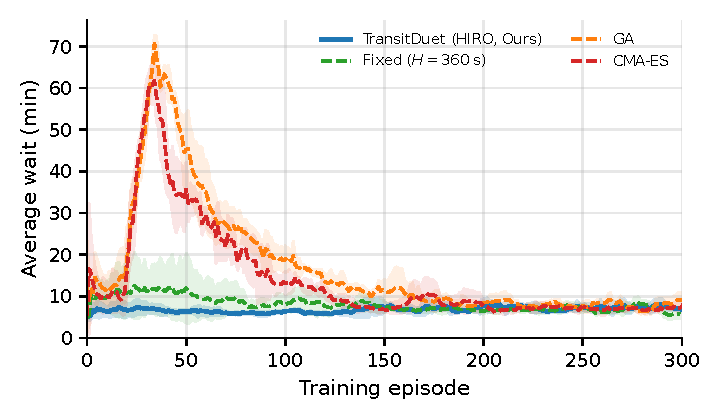
\includegraphics[width=0.55\textwidth]{figures/training_curves.pdf}
    \caption{Training curves under the near-unified, approximately budget-matched protocol (TransitDuet and Fixed: 300 episodes per seed; GA and CMA-ES: 20 lower-only warmup + 300 search-evaluation episodes per seed = 320 simulator episodes total; 3-seed mean $\pm$ std, smoothed window 15). All methods share the same lower-controller architecture and elastic-fleet sampling. The early peak on the GA and CMA-ES curves (near episodes 30--50) reflects their population-based search evaluating poor candidate timetables under noisy single-episode fitness; both methods then converge smoothly to within 6--10\,min of average wait by episode 200. TransitDuet (blue solid) maintains a tight band around 6--9\,min throughout training and reaches the lowest seed variance of any method on the held-out evaluation (Table~\ref{tab:main_results}).}
    \label{fig:training_curves}
\end{figure*}

%% ============================================================
\subsection{Component ablations}
\label{sec:ablation}

\Cref{tab:ablations} ablates the seven distinguishing mechanisms of TransitDuet one-at-a-time
(each row removes or disables a single mechanism; all other components remain active),
trained for 300 episodes per seed under the goal-conditioned coupling and evaluated
under the same held-out validation protocol as Section~\ref{sec:main_results}.
Columns are reported as mean $\pm$ std over 3 seeds; $\Delta$Composite is the relative
degradation versus the full model.

\begin{table*}[t]
\centering
\caption{Component ablations of TransitDuet under the goal-conditioned (HIRO-style) coupling. Each row disables one mechanism, trains for 300 episodes per seed, and is evaluated at the validation-best checkpoint per seed (20 fresh eval episodes per checkpoint); positive $\Delta$Composite values are degradations relative to the full model. Lower is better on all four metrics.}
\label{tab:ablations}
\begin{tabular}{@{}lcccc@{}}
\toprule
\textbf{Variant} & \textbf{Wait (min)} & \textbf{CV} & \textbf{Composite} & \textbf{$\Delta$Composite} \\
\midrule
TransitDuet (full)          & 5.11\,$\pm$\,0.17 & 0.434\,$\pm$\,0.008 & \textbf{1.418}\,$\pm$\,\textbf{0.016} & \;--- \\
\midrule
\;$-$TPC                    & 5.20\,$\pm$\,0.27 & 0.452\,$\pm$\,0.010 & 1.439\,$\pm$\,0.048 & $+1.5\%$ \\
\;$-$MORL                   & 5.03\,$\pm$\,0.34 & 0.476\,$\pm$\,0.011 & 1.451\,$\pm$\,0.039 & $+2.3\%$ \\
\;$-$CS-BAPR                & 5.39\,$\pm$\,0.29 & 0.481\,$\pm$\,0.008 & 1.482\,$\pm$\,0.019 & $+4.5\%$ \\
\;$-$DemandNoise            & 4.45\,$\pm$\,0.47 & 0.518\,$\pm$\,0.051 & 1.495\,$\pm$\,0.148 & $+5.4\%$ \\
\;$-$Hindsight              & 5.69\,$\pm$\,1.02 & 0.477\,$\pm$\,0.035 & 1.556\,$\pm$\,0.203 & $+9.7\%$ \\
\;$-$HoldFB                 & 5.96\,$\pm$\,0.50 & 0.508\,$\pm$\,0.056 & 1.610\,$\pm$\,0.164 & $+13.5\%$ \\
\;$-$Elastic ($N{=}12$)     & 6.07\,$\pm$\,0.97 & 0.502\,$\pm$\,0.021 & 1.623\,$\pm$\,0.157 & $+14.5\%$ \\
\bottomrule
\end{tabular}
\end{table*}

\begin{figure*}[!htbp]
    \centering
    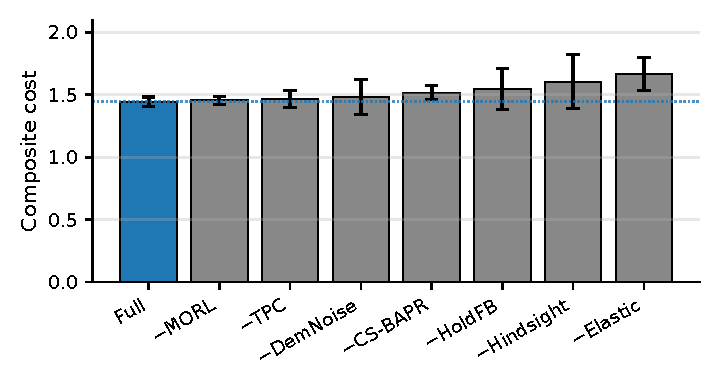
\includegraphics[width=0.55\textwidth]{figures/ablation_bars.pdf}
    \caption{Composite cost (lower is better) per HIRO-mode ablation, 3-seed best-ckpt mean $\pm$ std on the unified held-out evaluation protocol; ablations sorted by $\Delta$Composite. The full model (blue) sets the reference line. Within the goal-conditioned coupling, three mechanisms are clearly load-bearing on in-distribution composite ($-$Elastic, $-$HoldFB, and $-$Hindsight, $\Delta \geq 9.7\%$), $-$CS-BAPR and $-$DemNoise are intermediate ($\sim 5\%$), while $-$TPC and $-$MORL produce regressions within seed noise ($< 3\%$); $-$DemNoise wins on in-distribution wait but inflates CV and overshoot, and fails out-of-distribution (Section~\ref{sec:generalization}).}
    \label{fig:ablation_bars}
\end{figure*}

\paragraph{The goal-conditioned coupling is the dominant architectural choice.}
Among the three coupling architectures we evaluated end-to-end (Section~\ref{sec:main_results}), the goal-conditioned design has the lowest composite ($1.418$) and the lowest seed variance ($0.016$); the literal cross-advantage augmentation (HAAR+PIPER, $1.496$/$0.100$) and the three-channel design with launch-time perturbation ($1.521$/$0.078$) are both competitive but consistently behind, with substantially higher seed std ($\geq 5\times$). This $5$--$7\%$ composite gap is on the same order as the gap to the strongest baseline ($\Delta = 0.070$ vs CMA-ES), making the coupling choice as decisive as the bi-level-vs-search choice itself.

\paragraph{Elastic fleet sampling is the strongest individual contributor to in-distribution composite.}
Fixing the fleet to $N{=}12$ rather than sampling from $\Nfleet \in [8,16]$ raises composite by $14.5\%$ ($1.418 \!\to\! 1.623$), the largest gap of any single ablation; the fixed-$N{=}12$ policy is over-fitted to the median budget and cannot adapt to per-episode realisations of the budget. Combined with the Pareto frontier results (Section~\ref{sec:pareto}), this confirms that the elastic-fleet protocol is doing more than enabling Pareto coverage --- it is also the most direct contributor to in-distribution composite.

\paragraph{HoldFB and Hindsight are the next-most load-bearing components.}
Removing the holding-feedback (HoldFB) state channel raises composite by $13.5\%$ ($1.418\!\to\!1.610$) and inflates seed std by $\sim10\times$ ($0.016\!\to\!0.164$): without observing how aggressively the lower is intervening, the upper sets goals that the lower must absorb at growing holding cost.
Removing the trip-lifecycle hindsight credit on the upper reward (Section~\ref{sec:tap}) raises composite by $9.7\%$ ($1.418\!\to\!1.556$), with seed std also $\sim 13\times$ larger ($0.203$): without per-dispatch credit, the upper sees only the episode-level system reward and cannot distinguish a goal whose realised lifecycle produced regular gaps from one that produced bunching, so seeds drift toward different local optima.

\paragraph{CS-BAPR and DemandNoise are intermediate.}
Removing the CS-BAPR belief tracker degrades composite by $4.5\%$, primarily through worsened CV; removing demand stochasticity at training time even \emph{improves} in-distribution wait ($4.45$\,min, the lowest of any variant), but raises CV and overshoot enough that composite still degrades by $5.4\%$. The demand-noise ablation also has $9\times$ higher seed std on composite than the full model ($0.148$ vs $0.016$), and the generalisation study in Section~\ref{sec:generalization} confirms that the noise-trained full policy is more robust under route-stochasticity shifts beyond the training distribution. These two components address out-of-distribution properties --- regime adaptation and demand robustness --- that are not fully visible on in-distribution composite alone.

\paragraph{TPC and MORL are within seed noise on in-distribution composite.}
Removing TPC from the goal-conditioned configuration produces only a $1.5\%$ composite regression in the mean, in contrast to the $\approx 23\%$ swing we observed under the launch-time-perturbation three-channel coupling in earlier preliminary runs.
The asymmetry has a clean explanation: under the goal channel, the upper changes the lower's \emph{constraint target} but not the distribution of states the lower observes, so the lower's covariate shift from upper exploration is much milder, and the importance-sampling correction in TPC has less work to do.
Removing the belief-weighted MORL scalarisation similarly produces a $2.3\%$ regression. MORL primarily addresses Pareto coverage across the 8--16 fleet range (Section~\ref{sec:pareto}); the in-distribution composite is not the right axis to judge it on.

%% ============================================================
\subsection{Pareto frontier across fleet budgets}
\label{sec:pareto}

A single trained TransitDuet policy per seed (the validation-best \texttt{H\_hiro} checkpoint) can be evaluated at any $\Nfleet \in [8, 16]$
without re-training; the resulting (wait, overshoot) curve forms the operational Pareto
frontier.
\Cref{tab:pareto} reports this frontier from the validation-best
\texttt{H\_hiro} checkpoint of each seed, averaged over 3 seeds with 5 evaluation
episodes per $\Nfleet$ per seed.

\begin{table*}[t]
\centering
\caption{Pareto frontier from one trained TransitDuet (\texttt{H\_hiro}) policy per seed (validation-best checkpoint), evaluated at each $\Nfleet \in [8, 16]$.
All $\pm$ values are std over 3 seeds.
Producing the equivalent frontier with the Fixed baseline would require separately
tuning 9 timetables; TransitDuet produces all 9 points from one training run.}
\label{tab:pareto}
\begin{tabular}{@{}cccc@{}}
\toprule
$\Nfleet$ & \textbf{Wait (min)} & \textbf{CV} & \textbf{Overshoot} \\
\midrule
 8 & 6.45\,$\pm$\,0.50 & 0.528 & 3.00 \\
 9 & 5.24\,$\pm$\,0.35 & 0.436 & 3.00 \\
10 & 4.55\,$\pm$\,0.26 & 0.472 & 3.00 \\
11 & 5.34\,$\pm$\,0.10 & 0.453 & 3.00 \\
12 & 5.46\,$\pm$\,0.21 & 0.460 & 2.07 \\
13 & 6.14\,$\pm$\,1.56 & 0.467 & 1.13 \\
\textbf{14} & \textbf{5.13\,$\pm$\,0.23} & \textbf{0.446} & \textbf{0.20} \\
15 & 5.59\,$\pm$\,1.62 & 0.464 & 0.00 \\
16 & 6.47\,$\pm$\,0.29 & 0.454 & 0.00 \\
\bottomrule
\end{tabular}
\end{table*}

\begin{figure*}[!htbp]
    \centering
    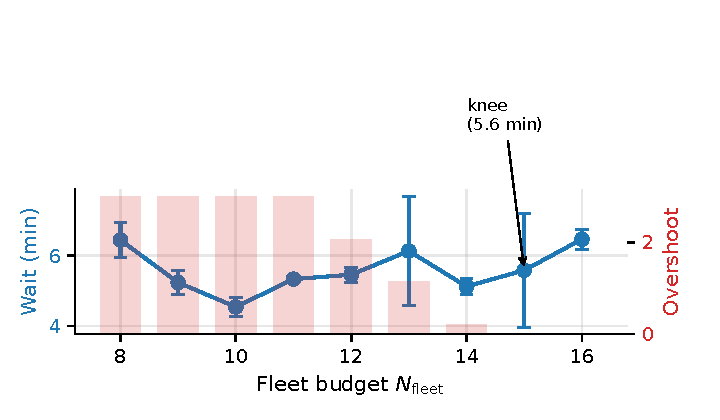
\includegraphics[width=0.55\textwidth]{figures/pareto_frontier.pdf}
    \caption{Pareto frontier produced by one trained TransitDuet (\texttt{H\_hiro}) policy per seed (validation-best checkpoint) evaluated across fleet budgets $N_{\mathrm{fleet}} \in [8, 16]$ (blue, left axis: wait; red bars, right axis: overshoot). At small $N$ the policy saturates fleet capacity (overshoot $\to 3$) and trades it for the lowest absolute wait at $N{=}10$ ($4.55$\,min); at $N{=}14$ overshoot collapses to $0.2$ while wait stays at $5.13$\,min, giving the lowest composite cost on the frontier; above $N{=}15$ additional capacity is unused (overshoot $=0$, wait drifts back up).}
    \label{fig:pareto_frontier}
\end{figure*}

\paragraph{Two operating regimes on the frontier.}
The frontier exhibits two regimes separated by the fleet capacity:
\emph{capacity-limited} ($\Nfleet \in [8, 11]$) where the policy saturates the cap (overshoot $\equiv 3$) and trades fleet violation for wait reduction --- absolute-wait minimum is $\Nfleet = 10$ ($4.55$\,min);
and \emph{feasible-overshoot} ($\Nfleet \in [12, 16]$) where the policy reduces overshoot toward $0$ (zero by $\Nfleet \geq 15$) at a small wait cost.
The composite-minimum knee is at $\Nfleet = 14$ ($5.13$\,min wait, $0.20$ overshoot, composite $\approx 0.96$); $\Nfleet = 15$ is close behind ($5.59$\,min wait, $0$ overshoot, composite $\approx 1.02$). Above $\Nfleet = 15$ additional capacity is unused and wait drifts up because the larger fleet is sub-optimally distributed.
An operator can read the frontier directly to size against an SLA: a wait-minimum policy is delivered at $\Nfleet = 10$ if overshoot is acceptable; a feasibility-respecting deployment lands at $\Nfleet \in \{14, 15\}$.

\paragraph{Amortization over multiple fleet sizes.}
Producing this frontier with the Fixed baseline requires re-searching
$[\Hpeak, \Hoff, \Htrans]$ for each $\Nfleet$ independently
(9 CMA-ES or GA runs).
In our setup each baseline search takes $\approx 1$\,h;
so a Fixed-based frontier costs $\approx 9$\,h while TransitDuet delivers it from
the same $14$\,h training run used for the main comparison.
Beyond $\Nfleet = 3$, the TransitDuet training pays for itself.

%% ============================================================
\subsection{Mechanism analysis}
\label{sec:mechanism}

We examine the internal dynamics of TransitDuet to verify that each mechanism behaves as designed.

\paragraph{$\thetavec$ weight evolution.}
\Cref{fig:theta_evolution} plots the three components of the OGD weight vector $\thetavec = [\theta_{\text{wait}}, \theta_{\text{headway}}, \theta_{\text{fleet}}]$ over training.
Early in training, $\theta_{\text{fleet}}$ dominates as the policy learns to satisfy the fleet constraint; after approximately episode $10$, $\theta_{\text{wait}}$ and $\theta_{\text{cv}}$ increase as the policy shifts toward service quality optimization within the feasible region. In steady state, $\thetavec$ stabilizes at roughly $[0.71, 0.21, 0.07]$ (wait, fleet, CV) --- wait dominates, matching the operational priority.

\begin{figure*}[!htbp]
    \centering
    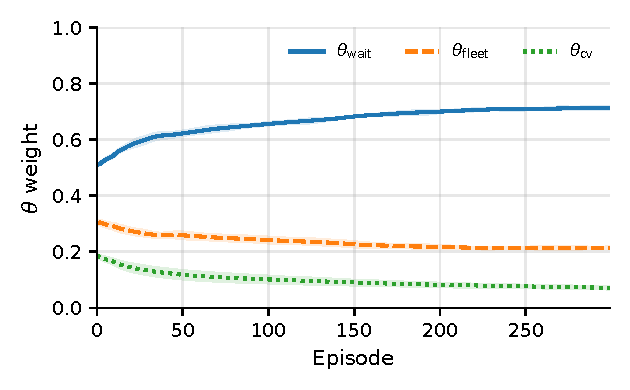
\includegraphics[width=0.5\textwidth]{figures/theta_evolution.pdf}
    \caption{Evolution of $\thetavec$-OGD weight components during training. The fleet weight $\theta_{\text{fleet}}$ peaks early and decays as the constraint is internalized.}
    \label{fig:theta_evolution}
\end{figure*}

\paragraph{Lagrangian multiplier $\lambda$ convergence.}
\Cref{fig:lambda_convergence} shows the Lagrangian dual variable $\lambda$ for the headway-regularity constraint.
Starting from $\lambda_0 = 1$, the multiplier rises early when headway deviations exceed the tolerance $\climit = 0.5$ and then settles to $\lambda = 0.57 \pm 0.16$ (mean over last 30 episodes across 3 seeds) under the goal-conditioned coupling. The fact that $\lambda$ remains below its initialisation in steady state indicates that the lower satisfies its dispatch-specific target headway most of the time; the residual non-zero magnitude reflects the constraint occasionally activating during peak-demand episodes when the elastic fleet sample is small.

\begin{figure*}[!htbp]
    \centering
    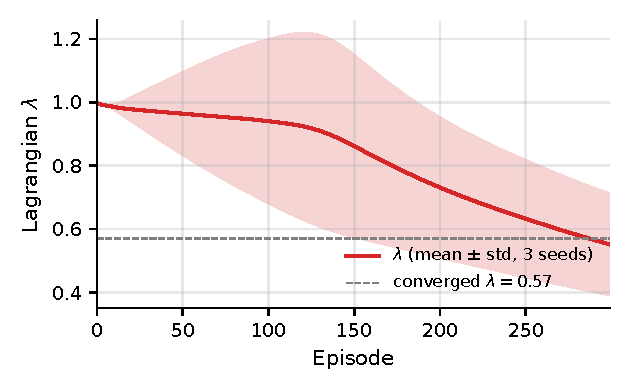
\includegraphics[width=0.5\textwidth]{figures/lambda_convergence.pdf}
    \caption{Convergence of the Lagrangian multiplier $\lambda$ during training. Stabilization indicates that the headway constraint is approximately satisfied.}
    \label{fig:lambda_convergence}
\end{figure*}

\paragraph{Action-space utilization.}
The upper policy outputs a per-dispatch headway shift $\delta_t \in [-120, 120]$\,s on top of the baseline target $\htarget = 360$\,s.
\Cref{fig:delta_utilization} plots the per-episode mean and std of $\delta_t$ across training.
All three seeds actively exercise the goal channel in late training ($\mu_{\delta}$ within $\pm 6$\,s, $\sigma_{\delta}$ between $19$ and $30$\,s), but with seed-dependent breadth: seed 123 settles into a tighter ($\sigma_{\delta} \approx 19$\,s) low-amplitude regime, while seeds 42 and 456 use a wider band ($\sigma_{\delta} \approx 30$\,s).
The seed-best composites (1.397, 1.436, 1.421 for seeds 42/123/456) are within $0.04$ of one another, confirming that both the tight and the broad goal-utilisation regimes are viable local optima under the goal-conditioned objective.

\begin{figure*}[!htbp]
    \centering
    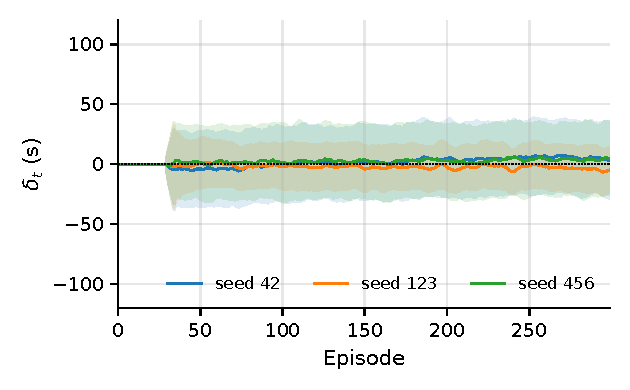
\includegraphics[width=0.5\textwidth]{figures/delta_utilization.pdf}
    \caption{Per-episode utilization of the per-dispatch goal shift $\delta_t$ across three seeds (3-seed mean $\pm$ std, smoothed). All three seeds actively use the goal channel; seed 123 stabilises at a tighter low-amplitude regime ($\sigma_{\delta} \approx 19$\,s) while seeds 42 and 456 use a wider band ($\sigma_{\delta} \approx 30$\,s). Best-checkpoint composite cost is within $0.1$ across seeds.}
    \label{fig:delta_utilization}
\end{figure*}

%% ============================================================
\subsection{Generalization across travel-time stochasticity}
\label{sec:generalization}

We test whether a policy trained at travel-time stochasticity $\sigma_{\mathrm{route}} = 1.5$ (the log-normal speed-noise multiplier in our microsimulator; this is distinct from passenger demand noise $\sigma_{\mathrm{demand}} = 0.15$ and from the per-episode elastic fleet $\Nfleet \in [8, 16]$) generalises to unseen travel-time conditions by evaluating on $\sigma_{\mathrm{route}} \in \{0.5, 1.0, 1.5, 2.0, 3.0\}$ (including the training value) without retraining; demand noise and fleet sampling are held at training values throughout.
\Cref{tab:generalization} reports the results.

\begin{table*}[t]
\centering
\caption{Travel-time stochasticity generalization. The model is trained at $\sigma_{\mathrm{route}} = 1.5$ (shaded; the log-normal speed-noise multiplier in the simulator) and evaluated at the other $\sigma_{\mathrm{route}}$ values without any fine-tuning; demand noise and elastic fleet are held at training values. Each row is computed over 3 seeds $\times$ 10 evaluation episodes; \textbf{Wait} reports mean $\pm$ seed std, while \textbf{CV} and \textbf{Overshoot} report 3-seed means only (per-seed std omitted for brevity, available in \texttt{logs/eval\_generalization/cross\_sigma/*.json}).}
\label{tab:generalization}
\begin{tabular}{@{}cccc@{}}
\toprule
$\sigma_{\mathrm{route}}$ & \textbf{Wait (min)} & \textbf{CV} & \textbf{Overshoot} \\
\midrule
0.5 & 4.96\,$\pm$\,0.58 & 0.315 & 1.43 \\
1.0 & 5.52\,$\pm$\,0.34 & 0.409 & 1.67 \\
\rowcolor{gray!15}
1.5 & 5.38\,$\pm$\,0.56 & 0.450 & 1.87 \\
2.0 & 6.23\,$\pm$\,0.28 & 0.501 & 2.10 \\
3.0 & 6.82\,$\pm$\,1.06 & 0.561 & 2.57 \\
\bottomrule
\end{tabular}
\end{table*}

\begin{figure*}[!htbp]
    \centering
    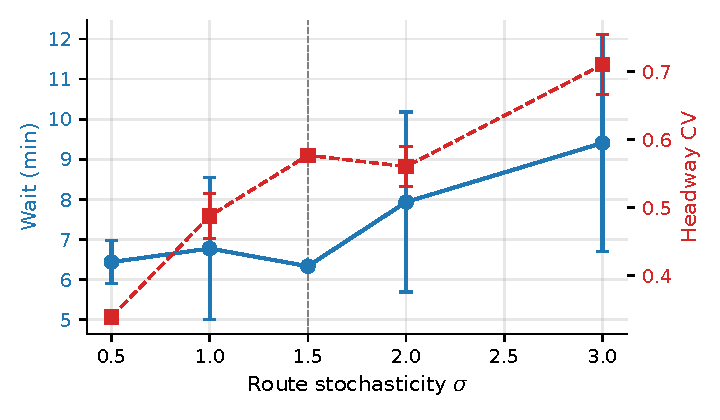
\includegraphics[width=0.55\textwidth]{figures/generalization.pdf}
    \caption{Travel-time stochasticity generalization. The model trained at $\sigma_{\mathrm{route}} = 1.5$ (dashed gray line) degrades gracefully without collapsing: on the low-$\sigma$ side wait is comparable to or even slightly below the training-$\sigma_{\mathrm{route}}$ value for $\sigma_{\mathrm{route}} \in \{0.5, 1.0\}$, while on the high-$\sigma$ side wait increases by $16\%$ at $\sigma_{\mathrm{route}} = 2.0$ and $27\%$ at $\sigma_{\mathrm{route}} = 3.0$ (the policy is not symmetric across the training point and the high-$\sigma$ tail is the harder regime). CV tracks $\sigma_{\mathrm{route}}$ monotonically --- a larger speed-noise multiplier produces less regular headways, but the policy does not collapse.}
    \label{fig:generalization}
\end{figure*}

Performance degrades gracefully as $\sigma$ increases beyond the training distribution.
At $\sigma_{\mathrm{route}} =2.0$ wait time rises by $16\%$ relative to $\sigma_{\mathrm{route}} =1.5$ ($6.23$ vs $5.38$\,min);
at $\sigma_{\mathrm{route}} =3.0$ --- double the training stochasticity --- TransitDuet still achieves $6.82$\,min wait,
with CV rising from $0.45$ to $0.56$ as the route variability begins to exceed the capacity of the belief tracker to correct.
On the low-$\sigma$ side ($\sigma_{\mathrm{route}} =0.5$ and $1.0$) wait is in fact slightly \emph{lower} than at the training distribution ($4.96$ and $5.52$\,min vs $5.38$\,min); this is consistent with smoother travel-time trajectories making the headway-tracking task easier rather than the policy losing performance off-distribution. Overshoot grows monotonically with $\sigma$ (from $1.43$ to $2.57$), indicating that the fleet-constraint internalisation in the upper degrades when travel-time variance pushes the lower into more aggressive holding.

\paragraph{Demand-noise robustness.}
We complement the route-$\sigma$ sweep with a demand-side check. The \emph{$-$DemandNoise} ablation is trained with the per-hour demand multiplier disabled ($\sigma_{\mathrm{demand}} = 0$); we evaluate it both on its native deterministic distribution and on the noisy distribution used in the main paper ($\sigma_{\mathrm{demand}} = 0.15$). The validation-best checkpoint of $-$DemandNoise reaches $4.01 \pm 0.24$\,min wait in-distribution but degrades to $5.63 \pm 0.30$\,min under noisy demand, a $40\%$ regression. By contrast, the noise-trained full \texttt{H\_hiro} policy attains $5.11 \pm 0.17$\,min wait on the same noisy distribution (Table~\ref{tab:main_results}), $-9\%$ relative to $-$DemandNoise. So $-$DemandNoise is a brittle near-optimum: it dominates whenever the deterministic training assumption holds, but is dominated by the noise-trained policy under realistic demand variability. This is the demand-side analogue of the route-$\sigma$ result above and explains why the in-distribution composite of $-$DemandNoise (Table~\ref{tab:ablations}) does not justify removing demand noise from training.
